% Options for packages loaded elsewhere
\PassOptionsToPackage{unicode}{hyperref}
\PassOptionsToPackage{hyphens}{url}
%
\documentclass[
]{article}
\usepackage{amsmath,amssymb}
\usepackage{iftex}
\ifPDFTeX
  \usepackage[T1]{fontenc}
  \usepackage[utf8]{inputenc}
  \usepackage{textcomp} % provide euro and other symbols
\else % if luatex or xetex
  \usepackage{unicode-math} % this also loads fontspec
  \defaultfontfeatures{Scale=MatchLowercase}
  \defaultfontfeatures[\rmfamily]{Ligatures=TeX,Scale=1}
\fi
\usepackage{lmodern}
\ifPDFTeX\else
  % xetex/luatex font selection
\fi
% Use upquote if available, for straight quotes in verbatim environments
\IfFileExists{upquote.sty}{\usepackage{upquote}}{}
\IfFileExists{microtype.sty}{% use microtype if available
  \usepackage[]{microtype}
  \UseMicrotypeSet[protrusion]{basicmath} % disable protrusion for tt fonts
}{}
\makeatletter
\@ifundefined{KOMAClassName}{% if non-KOMA class
  \IfFileExists{parskip.sty}{%
    \usepackage{parskip}
  }{% else
    \setlength{\parindent}{0pt}
    \setlength{\parskip}{6pt plus 2pt minus 1pt}}
}{% if KOMA class
  \KOMAoptions{parskip=half}}
\makeatother
\usepackage{xcolor}
\usepackage[margin=1in]{geometry}
\usepackage{color}
\usepackage{fancyvrb}
\newcommand{\VerbBar}{|}
\newcommand{\VERB}{\Verb[commandchars=\\\{\}]}
\DefineVerbatimEnvironment{Highlighting}{Verbatim}{commandchars=\\\{\}}
% Add ',fontsize=\small' for more characters per line
\usepackage{framed}
\definecolor{shadecolor}{RGB}{248,248,248}
\newenvironment{Shaded}{\begin{snugshade}}{\end{snugshade}}
\newcommand{\AlertTok}[1]{\textcolor[rgb]{0.94,0.16,0.16}{#1}}
\newcommand{\AnnotationTok}[1]{\textcolor[rgb]{0.56,0.35,0.01}{\textbf{\textit{#1}}}}
\newcommand{\AttributeTok}[1]{\textcolor[rgb]{0.13,0.29,0.53}{#1}}
\newcommand{\BaseNTok}[1]{\textcolor[rgb]{0.00,0.00,0.81}{#1}}
\newcommand{\BuiltInTok}[1]{#1}
\newcommand{\CharTok}[1]{\textcolor[rgb]{0.31,0.60,0.02}{#1}}
\newcommand{\CommentTok}[1]{\textcolor[rgb]{0.56,0.35,0.01}{\textit{#1}}}
\newcommand{\CommentVarTok}[1]{\textcolor[rgb]{0.56,0.35,0.01}{\textbf{\textit{#1}}}}
\newcommand{\ConstantTok}[1]{\textcolor[rgb]{0.56,0.35,0.01}{#1}}
\newcommand{\ControlFlowTok}[1]{\textcolor[rgb]{0.13,0.29,0.53}{\textbf{#1}}}
\newcommand{\DataTypeTok}[1]{\textcolor[rgb]{0.13,0.29,0.53}{#1}}
\newcommand{\DecValTok}[1]{\textcolor[rgb]{0.00,0.00,0.81}{#1}}
\newcommand{\DocumentationTok}[1]{\textcolor[rgb]{0.56,0.35,0.01}{\textbf{\textit{#1}}}}
\newcommand{\ErrorTok}[1]{\textcolor[rgb]{0.64,0.00,0.00}{\textbf{#1}}}
\newcommand{\ExtensionTok}[1]{#1}
\newcommand{\FloatTok}[1]{\textcolor[rgb]{0.00,0.00,0.81}{#1}}
\newcommand{\FunctionTok}[1]{\textcolor[rgb]{0.13,0.29,0.53}{\textbf{#1}}}
\newcommand{\ImportTok}[1]{#1}
\newcommand{\InformationTok}[1]{\textcolor[rgb]{0.56,0.35,0.01}{\textbf{\textit{#1}}}}
\newcommand{\KeywordTok}[1]{\textcolor[rgb]{0.13,0.29,0.53}{\textbf{#1}}}
\newcommand{\NormalTok}[1]{#1}
\newcommand{\OperatorTok}[1]{\textcolor[rgb]{0.81,0.36,0.00}{\textbf{#1}}}
\newcommand{\OtherTok}[1]{\textcolor[rgb]{0.56,0.35,0.01}{#1}}
\newcommand{\PreprocessorTok}[1]{\textcolor[rgb]{0.56,0.35,0.01}{\textit{#1}}}
\newcommand{\RegionMarkerTok}[1]{#1}
\newcommand{\SpecialCharTok}[1]{\textcolor[rgb]{0.81,0.36,0.00}{\textbf{#1}}}
\newcommand{\SpecialStringTok}[1]{\textcolor[rgb]{0.31,0.60,0.02}{#1}}
\newcommand{\StringTok}[1]{\textcolor[rgb]{0.31,0.60,0.02}{#1}}
\newcommand{\VariableTok}[1]{\textcolor[rgb]{0.00,0.00,0.00}{#1}}
\newcommand{\VerbatimStringTok}[1]{\textcolor[rgb]{0.31,0.60,0.02}{#1}}
\newcommand{\WarningTok}[1]{\textcolor[rgb]{0.56,0.35,0.01}{\textbf{\textit{#1}}}}
\usepackage{graphicx}
\makeatletter
\def\maxwidth{\ifdim\Gin@nat@width>\linewidth\linewidth\else\Gin@nat@width\fi}
\def\maxheight{\ifdim\Gin@nat@height>\textheight\textheight\else\Gin@nat@height\fi}
\makeatother
% Scale images if necessary, so that they will not overflow the page
% margins by default, and it is still possible to overwrite the defaults
% using explicit options in \includegraphics[width, height, ...]{}
\setkeys{Gin}{width=\maxwidth,height=\maxheight,keepaspectratio}
% Set default figure placement to htbp
\makeatletter
\def\fps@figure{htbp}
\makeatother
\setlength{\emergencystretch}{3em} % prevent overfull lines
\providecommand{\tightlist}{%
  \setlength{\itemsep}{0pt}\setlength{\parskip}{0pt}}
\setcounter{secnumdepth}{-\maxdimen} % remove section numbering
\usepackage{booktabs}
\usepackage{longtable}
\usepackage{array}
\usepackage{multirow}
\usepackage{wrapfig}
\usepackage{float}
\usepackage{colortbl}
\usepackage{pdflscape}
\usepackage{tabu}
\usepackage{threeparttable}
\usepackage{threeparttablex}
\usepackage[normalem]{ulem}
\usepackage{makecell}
\usepackage{xcolor}
\ifLuaTeX
  \usepackage{selnolig}  % disable illegal ligatures
\fi
\IfFileExists{bookmark.sty}{\usepackage{bookmark}}{\usepackage{hyperref}}
\IfFileExists{xurl.sty}{\usepackage{xurl}}{} % add URL line breaks if available
\urlstyle{same}
\hypersetup{
  pdftitle={Trabalho - Econometria IV},
  pdfauthor={Guilherme Luz, Guilherme Masuko, Caio Garzeri},
  hidelinks,
  pdfcreator={LaTeX via pandoc}}

\title{Trabalho - Econometria IV}
\author{Guilherme Luz, Guilherme Masuko, Caio Garzeri}
\date{August 2023}

\begin{document}
\maketitle

\begin{Shaded}
\begin{Highlighting}[]
\FunctionTok{library}\NormalTok{(lubridate)  }\CommentTok{\# for handling dates}
\FunctionTok{library}\NormalTok{(zoo)  }\CommentTok{\# for time series}
\FunctionTok{library}\NormalTok{(dynlm)  }\CommentTok{\# for time series regressions}
\FunctionTok{library}\NormalTok{(forecast)  }\CommentTok{\# for the improved Pacf function}
\FunctionTok{library}\NormalTok{(glmnet)  }\CommentTok{\# for shrinkage methods}
\FunctionTok{library}\NormalTok{(HDeconometrics)  }\CommentTok{\# IC for glmnet}

\CommentTok{\# Packages for parallel computation}
\FunctionTok{library}\NormalTok{(future)}
\FunctionTok{library}\NormalTok{(foreach)}
\FunctionTok{library}\NormalTok{(doFuture)}
\FunctionTok{library}\NormalTok{(doRNG)}
\end{Highlighting}
\end{Shaded}

\hypertarget{question-2}{%
\section{Question 2}\label{question-2}}

First of all, we must do some data wrangling.

\begin{Shaded}
\begin{Highlighting}[]
\CommentTok{\# Import the data}
\NormalTok{raw\_data }\OtherTok{=} \FunctionTok{read\_csv}\NormalTok{(}\StringTok{"data/2021{-}12.csv"}\NormalTok{)}
\NormalTok{data0 }\OtherTok{=}\NormalTok{ raw\_data[}\SpecialCharTok{{-}}\DecValTok{1}\NormalTok{, ] }\SpecialCharTok{\%\textgreater{}\%}
    \FunctionTok{select\_if}\NormalTok{(}\SpecialCharTok{\textasciitilde{}!}\FunctionTok{any}\NormalTok{(}\FunctionTok{is.na}\NormalTok{(.)))}
\NormalTok{transformation }\OtherTok{=}\NormalTok{ raw\_data[}\DecValTok{1}\NormalTok{, ]}
\end{Highlighting}
\end{Shaded}

The suggested transformations (in order to make the series stationary)
are indicated according to the following numeration.

Transformation codes (from FRED):

\begin{enumerate}
\def\labelenumi{\arabic{enumi}.}
\tightlist
\item
  no transformation
\item
  \(\Delta x_t\)
\item
  \(\Delta^2 x_t\)
\item
  \(\log(x_t)\)
\item
  \(\Delta \log(x_t)\)
\item
  \(\Delta^2 \log(x_t)\)
\item
  \(\Delta (x_t/x_{t-1} -1)\)
\end{enumerate}

For the CPI, we apply a specific transformation to turn it into an
inflation series.
\textcolor{blue}{Detalhe: estou usando a definição de inflação dada no enunciado $\pi_t = \frac{\Delta P_t}{P_t}$, que difere da definição usual $\pi_t = \frac{\Delta P_t}{P_{t-1}}$}

\begin{Shaded}
\begin{Highlighting}[]
\CommentTok{\# Data transformations based on the FRED transformation}
\CommentTok{\# codes}
\NormalTok{data }\OtherTok{=}\NormalTok{ data0 }\SpecialCharTok{\%\textgreater{}\%}
    \FunctionTok{select}\NormalTok{(}\SpecialCharTok{{-}}\NormalTok{sasdate) }\SpecialCharTok{\%\textgreater{}\%}
    \FunctionTok{rename}\NormalTok{(}\AttributeTok{SP500 =} \StringTok{"S\&P 500"}\NormalTok{, }\AttributeTok{SPINDUST =} \StringTok{"S\&P: indust"}\NormalTok{) }\SpecialCharTok{\%\textgreater{}\%}
\NormalTok{    BVAR}\SpecialCharTok{::}\FunctionTok{fred\_transform}\NormalTok{(}\AttributeTok{type =} \StringTok{"fred\_md"}\NormalTok{) }\SpecialCharTok{\%\textgreater{}\%}
    \FunctionTok{bind\_cols}\NormalTok{(}\FunctionTok{tibble}\NormalTok{(}\AttributeTok{date =}\NormalTok{ data0}\SpecialCharTok{$}\NormalTok{sasdate[}\DecValTok{3}\SpecialCharTok{:}\FunctionTok{length}\NormalTok{(data0}\SpecialCharTok{$}\NormalTok{sasdate)])) }\SpecialCharTok{\%\textgreater{}\%}
    \FunctionTok{mutate}\NormalTok{(}\AttributeTok{date =} \FunctionTok{as.Date}\NormalTok{(date, }\AttributeTok{format =} \StringTok{"\%m/\%d/\%Y"}\NormalTok{))}

\CommentTok{\# For the CPI, we transform into an inflation series}
\NormalTok{data }\OtherTok{=} \FunctionTok{mutate}\NormalTok{(data, }\AttributeTok{CPIAUCSL =} \DecValTok{100} \SpecialCharTok{*}\NormalTok{ (}\FunctionTok{diff}\NormalTok{(data0}\SpecialCharTok{$}\NormalTok{CPIAUCSL, }\AttributeTok{differences =} \DecValTok{1}\NormalTok{)}\SpecialCharTok{/}\NormalTok{data0}\SpecialCharTok{$}\NormalTok{CPIAUCSL[}\SpecialCharTok{{-}}\DecValTok{1}\NormalTok{])[}\SpecialCharTok{{-}}\DecValTok{1}\NormalTok{])}
\end{Highlighting}
\end{Shaded}

\begin{Shaded}
\begin{Highlighting}[]
\CommentTok{\# Inflation as time series}
\NormalTok{inflation }\OtherTok{=}\NormalTok{ data}\SpecialCharTok{$}\NormalTok{CPIAUCSL }\SpecialCharTok{\%\textgreater{}\%}
    \FunctionTok{ts}\NormalTok{(}\AttributeTok{start =} \FunctionTok{c}\NormalTok{(}\FunctionTok{year}\NormalTok{(data}\SpecialCharTok{$}\NormalTok{date[}\DecValTok{1}\NormalTok{]), }\FunctionTok{month}\NormalTok{(data}\SpecialCharTok{$}\NormalTok{date[}\DecValTok{1}\NormalTok{])), }\AttributeTok{frequency =} \DecValTok{12}\NormalTok{)}
\end{Highlighting}
\end{Shaded}

The resulting inflation series, which we want to forecast is shown
below.

\begin{Shaded}
\begin{Highlighting}[]
\CommentTok{\# plot inflation}

\NormalTok{data }\SpecialCharTok{\%\textgreater{}\%}
    \FunctionTok{select}\NormalTok{(date, CPIAUCSL) }\SpecialCharTok{\%\textgreater{}\%}
    \FunctionTok{mutate}\NormalTok{(}\AttributeTok{date =} \FunctionTok{as.Date}\NormalTok{(date, }\AttributeTok{format =} \StringTok{"\%m/\%d/\%Y"}\NormalTok{)) }\SpecialCharTok{\%\textgreater{}\%}
    \CommentTok{\# filter(date\textgreater{}as.Date(\textquotesingle{}2000{-}01{-}01\textquotesingle{})) \%\textgreater{}\%}
\FunctionTok{ggplot}\NormalTok{(}\FunctionTok{aes}\NormalTok{(}\AttributeTok{x =}\NormalTok{ date, }\AttributeTok{y =}\NormalTok{ CPIAUCSL)) }\SpecialCharTok{+} \FunctionTok{geom\_line}\NormalTok{() }\SpecialCharTok{+} \FunctionTok{labs}\NormalTok{(}\AttributeTok{title =} \StringTok{"Inflation (CPI, \% mom)"}\NormalTok{,}
    \AttributeTok{x =} \ConstantTok{NULL}\NormalTok{, }\AttributeTok{y =} \ConstantTok{NULL}\NormalTok{)}
\end{Highlighting}
\end{Shaded}

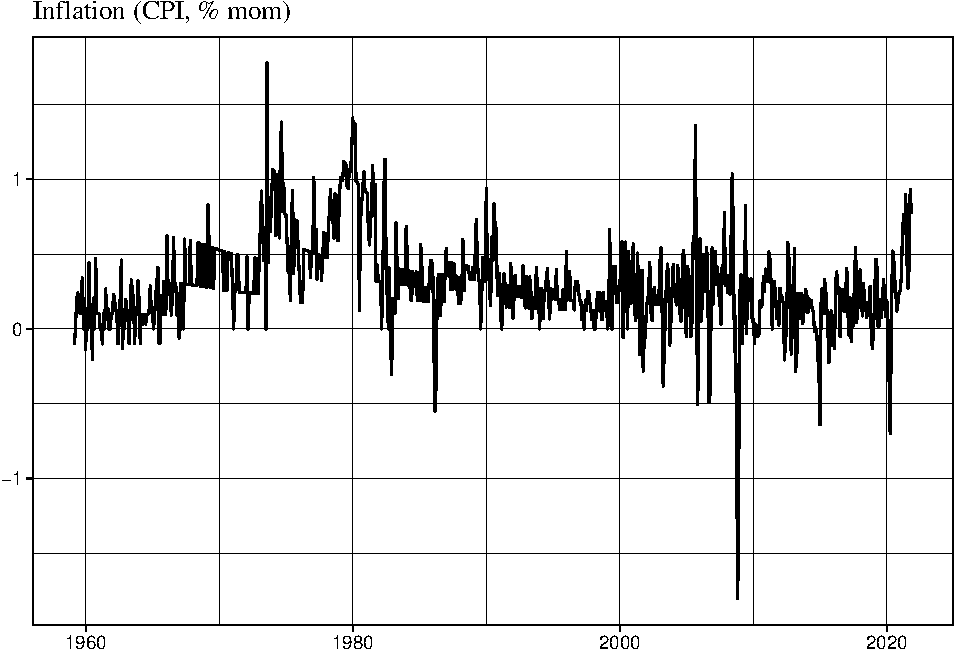
\includegraphics{Trabalho_Econo4_Q2_junto_files/figure-latex/unnamed-chunk-5-1.pdf}

Now, we shall start the estimations.

\hypertarget{ar}{%
\subsubsection{AR}\label{ar}}

In order to get some idea of what the order of our AR(p) process is, we
plot the partial autocorrelation of the inflation series for a
particular window.

\begin{Shaded}
\begin{Highlighting}[]
\CommentTok{\# Partial autocorrelation}
\NormalTok{inflation }\SpecialCharTok{\%\textgreater{}\%}
    \FunctionTok{window}\NormalTok{(}\AttributeTok{start =} \FunctionTok{start}\NormalTok{(inflation), }\AttributeTok{end =} \FunctionTok{start}\NormalTok{(inflation) }\SpecialCharTok{+}
        \FunctionTok{c}\NormalTok{(}\DecValTok{0}\NormalTok{, }\DecValTok{492}\NormalTok{)) }\SpecialCharTok{\%\textgreater{}\%}
    \FunctionTok{Pacf}\NormalTok{(}\AttributeTok{lag.max =} \DecValTok{24}\NormalTok{, }\AttributeTok{plot =}\NormalTok{ T)}
\end{Highlighting}
\end{Shaded}

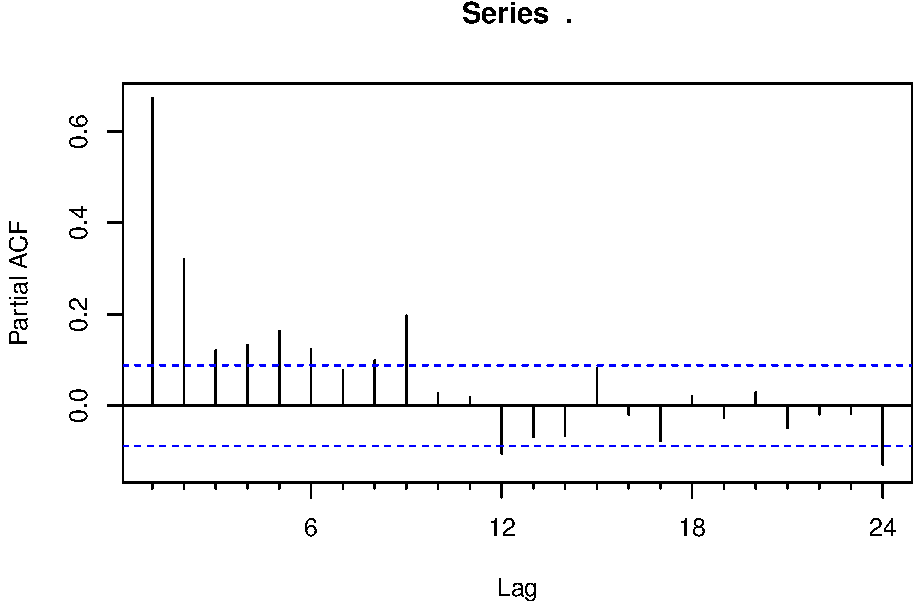
\includegraphics{Trabalho_Econo4_Q2_junto_files/figure-latex/unnamed-chunk-6-1.pdf}

We believe that a maximum lag of 24 is more than reasonable. Then, the
determine the actual order p based on the BIC.

\begin{Shaded}
\begin{Highlighting}[]
\CommentTok{\# Function for calculating the BIC for AR models}
\NormalTok{BIC.ar }\OtherTok{\textless{}{-}} \ControlFlowTok{function}\NormalTok{(model) \{}

\NormalTok{    ssr }\OtherTok{\textless{}{-}} \FunctionTok{sum}\NormalTok{(model}\SpecialCharTok{$}\NormalTok{resid}\SpecialCharTok{\^{}}\DecValTok{2}\NormalTok{, }\AttributeTok{na.rm =}\NormalTok{ T)}
\NormalTok{    t }\OtherTok{\textless{}{-}} \FunctionTok{length}\NormalTok{(model}\SpecialCharTok{$}\NormalTok{resid)}
\NormalTok{    npar }\OtherTok{\textless{}{-}} \FunctionTok{length}\NormalTok{(model}\SpecialCharTok{$}\NormalTok{coef)}

    \FunctionTok{return}\NormalTok{(}\FunctionTok{c}\NormalTok{(}\AttributeTok{p =}\NormalTok{ model}\SpecialCharTok{$}\NormalTok{order, }\AttributeTok{BIC =} \FunctionTok{log}\NormalTok{(ssr}\SpecialCharTok{/}\NormalTok{t) }\SpecialCharTok{+}\NormalTok{ npar }\SpecialCharTok{*} \FunctionTok{log}\NormalTok{(t)}\SpecialCharTok{/}\NormalTok{t))}
\NormalTok{\}}
\end{Highlighting}
\end{Shaded}

We proceed with a rolling window one-step-ahead forecast, in which we
choose the optimal order of the AR in each window of estimation.

\begin{Shaded}
\begin{Highlighting}[]
\CommentTok{\# Rolling window forecasting}
\NormalTok{rolling\_window }\OtherTok{\textless{}{-}} \DecValTok{492}
\NormalTok{p.max }\OtherTok{\textless{}{-}} \DecValTok{24}

\NormalTok{forecast1 }\OtherTok{=} \FunctionTok{list}\NormalTok{()}

\ControlFlowTok{for}\NormalTok{ (a }\ControlFlowTok{in} \DecValTok{0}\SpecialCharTok{:}\NormalTok{(}\FunctionTok{length}\NormalTok{(inflation) }\SpecialCharTok{{-}}\NormalTok{ rolling\_window }\SpecialCharTok{{-}} \DecValTok{1}\NormalTok{)) \{}

    \CommentTok{\# get the window for training the model}
\NormalTok{    train }\OtherTok{=} \FunctionTok{window}\NormalTok{(inflation, }\AttributeTok{start =} \FunctionTok{start}\NormalTok{(inflation) }\SpecialCharTok{+} \FunctionTok{c}\NormalTok{(}\DecValTok{0}\NormalTok{,}
\NormalTok{        a), }\AttributeTok{end =} \FunctionTok{start}\NormalTok{(inflation) }\SpecialCharTok{+} \FunctionTok{c}\NormalTok{(}\DecValTok{0}\NormalTok{, a }\SpecialCharTok{+}\NormalTok{ rolling\_window }\SpecialCharTok{{-}}
        \DecValTok{1}\NormalTok{))}
    \CommentTok{\# test = window(inflation, start =}
    \CommentTok{\# start(inflation)+c(0,a+rolling\_window), end =}
    \CommentTok{\# start(inflation)+c(0,a+rolling\_window))}

\NormalTok{    bic.table }\OtherTok{=} \FunctionTok{c}\NormalTok{()}

    \ControlFlowTok{for}\NormalTok{ (p }\ControlFlowTok{in} \DecValTok{0}\SpecialCharTok{:}\NormalTok{p.max) \{}
        \CommentTok{\# calculating the BIC for different orders of the}
        \CommentTok{\# AR(p)}
\NormalTok{        AR }\OtherTok{=} \FunctionTok{ar}\NormalTok{(train, }\AttributeTok{order.max =}\NormalTok{ p, }\AttributeTok{method =} \StringTok{"ols"}\NormalTok{, }\AttributeTok{aic =}\NormalTok{ F)}
\NormalTok{        bic.line }\OtherTok{=} \FunctionTok{BIC.ar}\NormalTok{(AR)}
\NormalTok{        bic.table }\OtherTok{=} \FunctionTok{rbind}\NormalTok{(bic.table, bic.line)}
\NormalTok{    \}}
\NormalTok{    bic.table }\OtherTok{=} \FunctionTok{data.frame}\NormalTok{(bic.table)}

\NormalTok{    p.opt }\OtherTok{=}\NormalTok{ bic.table}\SpecialCharTok{$}\NormalTok{p[}\FunctionTok{which.min}\NormalTok{(bic.table}\SpecialCharTok{$}\NormalTok{BIC)]  }\CommentTok{\# pick the optimal p}

\NormalTok{    AR }\OtherTok{=} \FunctionTok{ar}\NormalTok{(train, }\AttributeTok{order.max =}\NormalTok{ p.opt, }\AttributeTok{method =} \StringTok{"ols"}\NormalTok{, }\AttributeTok{aic =}\NormalTok{ F)  }\CommentTok{\# run the AR model with the optimal p}

\NormalTok{    forecast1[[a }\SpecialCharTok{+} \DecValTok{1}\NormalTok{]] }\OtherTok{=} \FunctionTok{predict}\NormalTok{(AR, }\AttributeTok{n.ahead =} \DecValTok{1}\NormalTok{)}\SpecialCharTok{$}\NormalTok{pred  }\CommentTok{\# one{-}step{-}ahead forecast}
\NormalTok{\}}

\NormalTok{forecasts }\OtherTok{=}\NormalTok{ forecast1 }\SpecialCharTok{\%\textgreater{}\%}
    \FunctionTok{unlist}\NormalTok{() }\SpecialCharTok{\%\textgreater{}\%}
    \FunctionTok{ts}\NormalTok{(}\AttributeTok{start =} \FunctionTok{start}\NormalTok{(forecast1[[}\DecValTok{1}\NormalTok{]]), }\AttributeTok{frequency =} \FunctionTok{frequency}\NormalTok{(forecast1[[}\DecValTok{1}\NormalTok{]]))}
\end{Highlighting}
\end{Shaded}

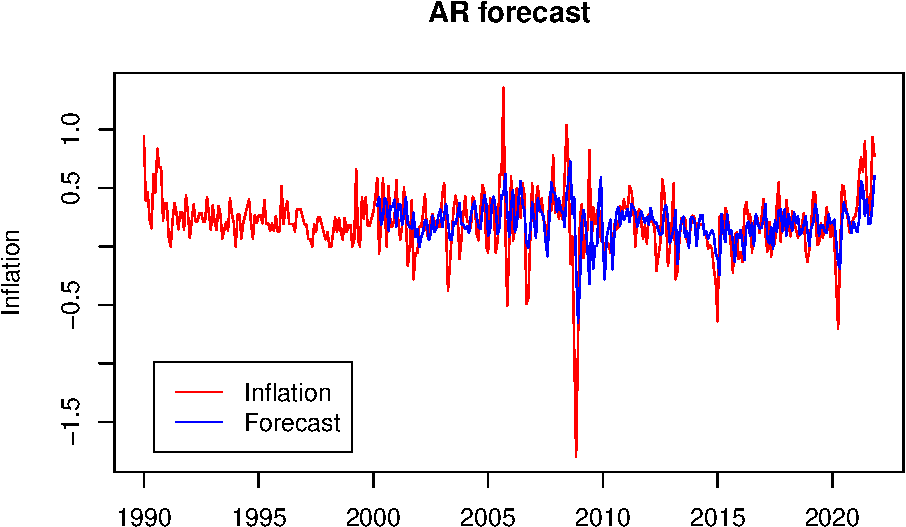
\includegraphics{Trabalho_Econo4_Q2_junto_files/figure-latex/unnamed-chunk-9-1.pdf}

\hypertarget{ar-pc}{%
\subsubsection{AR + PC}\label{ar-pc}}

\begin{enumerate}
\def\labelenumi{\arabic{enumi}.}
\tightlist
\item
  PCA
\end{enumerate}

We do a Principal Component Analysis (PCA). Note that we must center and
scale the data, since the series are in different scales.
\textcolor{red}{depois pra fazer previsao deveria me preocupar com isso?}

\begin{Shaded}
\begin{Highlighting}[]
\CommentTok{\# PCA}
\NormalTok{pca }\OtherTok{=}\NormalTok{ data }\SpecialCharTok{\%\textgreater{}\%}
    \FunctionTok{select}\NormalTok{(}\SpecialCharTok{{-}}\NormalTok{CPIAUCSL, }\SpecialCharTok{{-}}\NormalTok{date) }\SpecialCharTok{\%\textgreater{}\%}
    \FunctionTok{prcomp}\NormalTok{(}\AttributeTok{center =} \ConstantTok{TRUE}\NormalTok{, }\AttributeTok{scale =} \ConstantTok{TRUE}\NormalTok{)}
\end{Highlighting}
\end{Shaded}

\begin{enumerate}
\def\labelenumi{\arabic{enumi}.}
\setcounter{enumi}{1}
\tightlist
\item
  Select PCs
\end{enumerate}

We can, then, choose the number of factors \(k\) and select the first
\(k\) PCs. As seen in Question 1, there are different ways to choose the
number of factors. We look at 3 common criterion (rule of thumb,
informal way and biggest drop), but we opt for the rule of thumb as it
seems to be the most parsimonious in this case.
\textcolor{blue}{colocar alguma explicacao de qual criterio vamos adotar - usar rule of thumb q foi oq o masuko usou na 1}

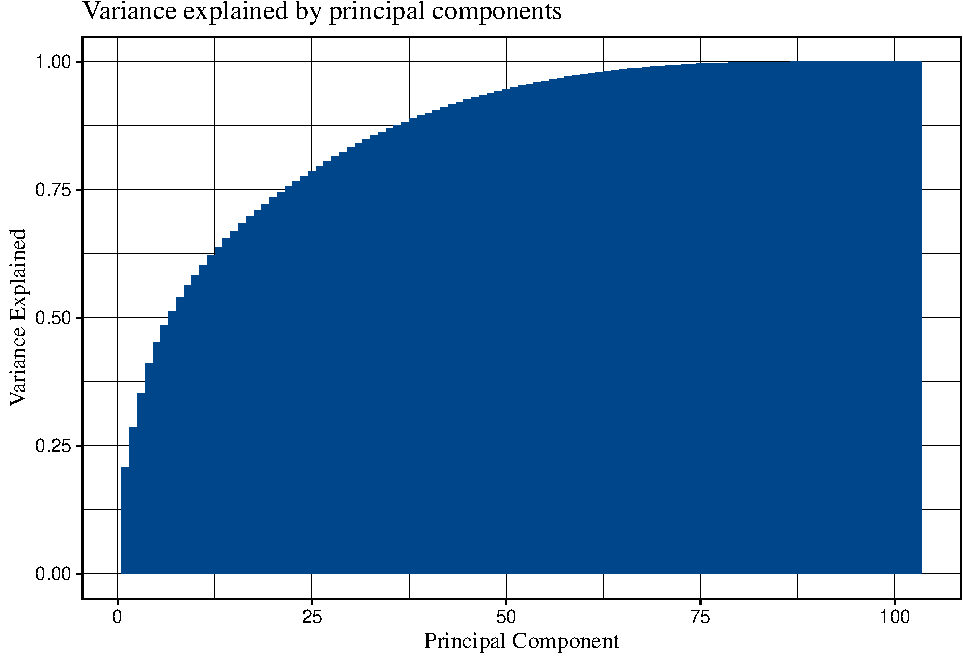
\includegraphics{Trabalho_Econo4_Q2_junto_files/figure-latex/unnamed-chunk-11-1.pdf}

\begin{Shaded}
\begin{Highlighting}[]
\CommentTok{\# Choosing the number of PCs}

\CommentTok{\# Rule of thumb (3\%)}

\NormalTok{pca.var.prop }\SpecialCharTok{\%\textgreater{}\%}
    \FunctionTok{filter}\NormalTok{(var.prop }\SpecialCharTok{\textgreater{}=} \FloatTok{0.03}\NormalTok{) }\SpecialCharTok{\%\textgreater{}\%}
    \FunctionTok{nrow}\NormalTok{() }\SpecialCharTok{\%\textgreater{}\%}
    \FunctionTok{paste}\NormalTok{(}\StringTok{"(rule of thumb)"}\NormalTok{)}
\end{Highlighting}
\end{Shaded}

\begin{verbatim}
## [1] "6 (rule of thumb)"
\end{verbatim}

\begin{Shaded}
\begin{Highlighting}[]
\CommentTok{\# Informal way (90\%)}

\NormalTok{pca.var.prop }\SpecialCharTok{\%\textgreater{}\%}
    \FunctionTok{filter}\NormalTok{(var.prop.cum }\SpecialCharTok{\textless{}=} \FloatTok{0.9}\NormalTok{) }\SpecialCharTok{\%\textgreater{}\%}
    \FunctionTok{nrow}\NormalTok{() }\SpecialCharTok{\%\textgreater{}\%}
    \FunctionTok{paste}\NormalTok{(}\StringTok{"(informal way)"}\NormalTok{)}
\end{Highlighting}
\end{Shaded}

\begin{verbatim}
## [1] "40 (informal way)"
\end{verbatim}

\begin{Shaded}
\begin{Highlighting}[]
\CommentTok{\# Biggest drop}

\NormalTok{(}\FunctionTok{lag}\NormalTok{(pca.var.prop}\SpecialCharTok{$}\NormalTok{var.prop)}\SpecialCharTok{/}\NormalTok{pca.var.prop}\SpecialCharTok{$}\NormalTok{var.prop) }\SpecialCharTok{\%\textgreater{}\%}
    \FunctionTok{which.max}\NormalTok{() }\SpecialCharTok{\%\textgreater{}\%}
    \SpecialCharTok{{-}}\DecValTok{1} \SpecialCharTok{\%\textgreater{}\%}
    \FunctionTok{paste}\NormalTok{(}\StringTok{"(biggest drop)"}\NormalTok{)}
\end{Highlighting}
\end{Shaded}

\begin{verbatim}
## [1] "102 (biggest drop)"
\end{verbatim}

\begin{Shaded}
\begin{Highlighting}[]
\CommentTok{\# Using the rule of thumb}
\NormalTok{n\_pc }\OtherTok{=}\NormalTok{ pca.var.prop }\SpecialCharTok{\%\textgreater{}\%}
    \FunctionTok{filter}\NormalTok{(var.prop }\SpecialCharTok{\textgreater{}=} \FloatTok{0.03}\NormalTok{) }\SpecialCharTok{\%\textgreater{}\%}
    \FunctionTok{nrow}\NormalTok{()}
\end{Highlighting}
\end{Shaded}

\begin{enumerate}
\def\labelenumi{\arabic{enumi}.}
\setcounter{enumi}{2}
\tightlist
\item
  Regression
\end{enumerate}

Given the number of factors, the order of the autoregressive component
is determined by BIC in each rolling window.

\begin{Shaded}
\begin{Highlighting}[]
\CommentTok{\# Get the factor from the PCA}
\NormalTok{Factors }\OtherTok{=}\NormalTok{ pca}\SpecialCharTok{$}\NormalTok{x[, }\DecValTok{1}\SpecialCharTok{:}\NormalTok{n\_pc]}

\CommentTok{\# Create the data matrix with the factors}
\NormalTok{variables }\OtherTok{=} \FunctionTok{cbind}\NormalTok{(inflation, Factors)}

\NormalTok{variables\_withdate }\OtherTok{=}\NormalTok{ variables }\SpecialCharTok{\%\textgreater{}\%}
    \FunctionTok{bind\_cols}\NormalTok{(}\AttributeTok{date =} \FunctionTok{as.Date.yearmon}\NormalTok{(}\FunctionTok{time}\NormalTok{(inflation))) }\SpecialCharTok{\%\textgreater{}\%}
    \FunctionTok{setNames}\NormalTok{(}\FunctionTok{c}\NormalTok{(}\StringTok{"inflation"}\NormalTok{, }\FunctionTok{colnames}\NormalTok{(Factors), }\StringTok{"date"}\NormalTok{))}
\end{Highlighting}
\end{Shaded}

We proceed with the rolling window one-step-ahead forecast.

\begin{Shaded}
\begin{Highlighting}[]
\CommentTok{\# Function for creating the proper data matrix based on the}
\CommentTok{\# regression formula}

\CommentTok{\# Instead of manually creating data matrix, we use the}
\CommentTok{\# dynlm() function and get only the $model component}
\NormalTok{create\_datamatrix }\OtherTok{=} \ControlFlowTok{function}\NormalTok{(train, p.opt) \{}
\NormalTok{    new }\OtherTok{=} \FunctionTok{dynlm}\NormalTok{(inflation }\SpecialCharTok{\textasciitilde{}} \FunctionTok{L}\NormalTok{(inflation, }\DecValTok{1}\SpecialCharTok{:}\NormalTok{p.opt) }\SpecialCharTok{+} \FunctionTok{L}\NormalTok{(train[,}
        \SpecialCharTok{{-}}\DecValTok{1}\NormalTok{], }\DecValTok{1}\NormalTok{), }\AttributeTok{data =} \FunctionTok{ts}\NormalTok{(}\FunctionTok{rbind}\NormalTok{(train, }\DecValTok{0}\NormalTok{), }\AttributeTok{start =} \FunctionTok{start}\NormalTok{(train),}
        \AttributeTok{frequency =} \FunctionTok{frequency}\NormalTok{(train)))}
\NormalTok{    new }\OtherTok{=}\NormalTok{ new}\SpecialCharTok{$}\NormalTok{model }\SpecialCharTok{\%\textgreater{}\%}
        \FunctionTok{tail}\NormalTok{(}\DecValTok{1}\NormalTok{) }\SpecialCharTok{\%\textgreater{}\%}
        \FunctionTok{select}\NormalTok{(}\SpecialCharTok{{-}}\NormalTok{inflation) }\SpecialCharTok{\%\textgreater{}\%}
        \FunctionTok{as.matrix}\NormalTok{()}
    \FunctionTok{return}\NormalTok{(new)}
\NormalTok{\}}
\end{Highlighting}
\end{Shaded}

\textcolor{red}{paralelizar esse pedaco pra rodar mais rapido; acho q nao precisa do test nesse pedaco tambem. Se nao precisar entao ja tira daqui e do chunk do AR}

\begin{Shaded}
\begin{Highlighting}[]
\CommentTok{\# Rolling window forecasting}
\NormalTok{rolling\_window }\OtherTok{\textless{}{-}} \DecValTok{492}
\NormalTok{p.max }\OtherTok{\textless{}{-}} \DecValTok{24}

\NormalTok{forecast1 }\OtherTok{=} \FunctionTok{list}\NormalTok{()}

\ControlFlowTok{for}\NormalTok{ (a }\ControlFlowTok{in} \DecValTok{0}\SpecialCharTok{:}\NormalTok{(}\FunctionTok{length}\NormalTok{(inflation) }\SpecialCharTok{{-}}\NormalTok{ rolling\_window }\SpecialCharTok{{-}} \DecValTok{1}\NormalTok{)) \{}

\NormalTok{    train }\OtherTok{=} \FunctionTok{window}\NormalTok{(variables, }\AttributeTok{start =} \FunctionTok{start}\NormalTok{(inflation) }\SpecialCharTok{+} \FunctionTok{c}\NormalTok{(}\DecValTok{0}\NormalTok{,}
\NormalTok{        a), }\AttributeTok{end =} \FunctionTok{start}\NormalTok{(inflation) }\SpecialCharTok{+} \FunctionTok{c}\NormalTok{(}\DecValTok{0}\NormalTok{, a }\SpecialCharTok{+}\NormalTok{ rolling\_window }\SpecialCharTok{{-}}
        \DecValTok{1}\NormalTok{))}
\NormalTok{    test }\OtherTok{=} \FunctionTok{window}\NormalTok{(variables, }\AttributeTok{start =} \FunctionTok{start}\NormalTok{(inflation) }\SpecialCharTok{+} \FunctionTok{c}\NormalTok{(}\DecValTok{0}\NormalTok{,}
\NormalTok{        a }\SpecialCharTok{+}\NormalTok{ rolling\_window), }\AttributeTok{end =} \FunctionTok{start}\NormalTok{(inflation) }\SpecialCharTok{+} \FunctionTok{c}\NormalTok{(}\DecValTok{0}\NormalTok{, a }\SpecialCharTok{+}
\NormalTok{        rolling\_window))}

\NormalTok{    bic.table }\OtherTok{=} \FunctionTok{rep}\NormalTok{(}\ConstantTok{NA}\NormalTok{, p.max)}

    \ControlFlowTok{for}\NormalTok{ (p }\ControlFlowTok{in} \DecValTok{1}\SpecialCharTok{:}\NormalTok{p.max) \{}
        \CommentTok{\# calculating the BIC for different orders of the}
        \CommentTok{\# AR(p)}
\NormalTok{        AR\_PC }\OtherTok{=} \FunctionTok{dynlm}\NormalTok{(inflation }\SpecialCharTok{\textasciitilde{}} \FunctionTok{L}\NormalTok{(inflation, }\DecValTok{1}\SpecialCharTok{:}\NormalTok{p) }\SpecialCharTok{+} \FunctionTok{L}\NormalTok{(train[,}
            \SpecialCharTok{{-}}\DecValTok{1}\NormalTok{], }\DecValTok{1}\NormalTok{), }\AttributeTok{data =}\NormalTok{ train)}
\NormalTok{        bic.table[p] }\OtherTok{=} \FunctionTok{BIC}\NormalTok{(AR\_PC)}
\NormalTok{    \}}

\NormalTok{    p.opt }\OtherTok{=} \FunctionTok{which.min}\NormalTok{(bic.table)  }\CommentTok{\# pick the optimal p}

\NormalTok{    AR\_PC }\OtherTok{=} \FunctionTok{dynlm}\NormalTok{(inflation }\SpecialCharTok{\textasciitilde{}} \FunctionTok{L}\NormalTok{(inflation, }\DecValTok{1}\SpecialCharTok{:}\NormalTok{p.opt) }\SpecialCharTok{+} \FunctionTok{L}\NormalTok{(train[,}
        \SpecialCharTok{{-}}\DecValTok{1}\NormalTok{], }\DecValTok{1}\NormalTok{), }\AttributeTok{data =}\NormalTok{ train)  }\CommentTok{\# run the AR{-}PC model with the optimal p}

\NormalTok{    new }\OtherTok{=} \FunctionTok{create\_datamatrix}\NormalTok{(train, p.opt)}

\NormalTok{    forecast1[[a }\SpecialCharTok{+} \DecValTok{1}\NormalTok{]] }\OtherTok{=}\NormalTok{ AR\_PC}\SpecialCharTok{$}\NormalTok{coefficients }\SpecialCharTok{\%*\%} \FunctionTok{c}\NormalTok{(}\DecValTok{1}\NormalTok{, new)  }\CommentTok{\# one{-}step{-}ahead forecast}
\NormalTok{\}}

\NormalTok{forecast1 }\OtherTok{=}\NormalTok{ forecast1 }\SpecialCharTok{\%\textgreater{}\%}
    \FunctionTok{unlist}\NormalTok{() }\SpecialCharTok{\%\textgreater{}\%}
    \FunctionTok{ts}\NormalTok{(}\AttributeTok{start =} \FunctionTok{start}\NormalTok{(inflation) }\SpecialCharTok{+} \FunctionTok{c}\NormalTok{(}\DecValTok{0}\NormalTok{, rolling\_window), }\AttributeTok{frequency =} \FunctionTok{frequency}\NormalTok{(inflation))}
\end{Highlighting}
\end{Shaded}

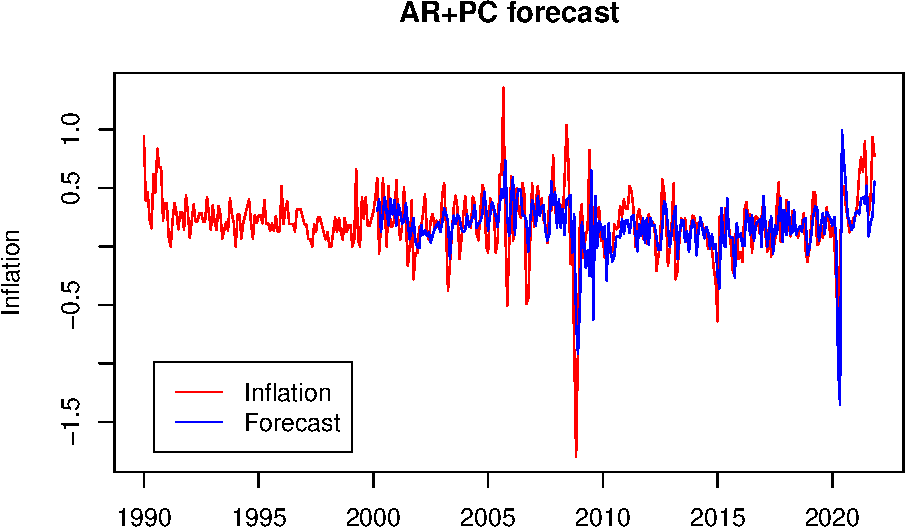
\includegraphics{Trabalho_Econo4_Q2_junto_files/figure-latex/unnamed-chunk-17-1.pdf}

\begin{Shaded}
\begin{Highlighting}[]
\CommentTok{\# Save forecasts}
\NormalTok{forecasts }\OtherTok{=} \FunctionTok{cbind}\NormalTok{(}\AttributeTok{AR =}\NormalTok{ forecasts, }\AttributeTok{AR\_PC =}\NormalTok{ forecast1) }\SpecialCharTok{\%\textgreater{}\%}
    \FunctionTok{as.ts}\NormalTok{()}
\end{Highlighting}
\end{Shaded}

\hypertarget{ridge-regression}{%
\subsubsection{Ridge Regression}\label{ridge-regression}}

We will choose penalty term according to the BIC. However, we must
decide on the number of lags in the model and this criterion is
obviously silent about this issue. Our strategy will be to run the
models with 1, 2, 3 and 4 lags and choose the model with the smallest
MSE.

\begin{Shaded}
\begin{Highlighting}[]
\CommentTok{\# Embedding}
\NormalTok{my\_embed }\OtherTok{=} \ControlFlowTok{function}\NormalTok{(df, }\AttributeTok{n\_lags =} \DecValTok{4}\NormalTok{) \{}
\NormalTok{    Lags }\OtherTok{=} \FunctionTok{list}\NormalTok{()}
\NormalTok{    Lags[[}\DecValTok{1}\NormalTok{]] }\OtherTok{=}\NormalTok{ df }\SpecialCharTok{\%\textgreater{}\%}
        \FunctionTok{select}\NormalTok{(}\SpecialCharTok{{-}}\FunctionTok{contains}\NormalTok{(}\StringTok{"date"}\NormalTok{))}
    \ControlFlowTok{for}\NormalTok{ (i }\ControlFlowTok{in} \DecValTok{1}\SpecialCharTok{:}\NormalTok{n\_lags) \{}
\NormalTok{        Lags[[i }\SpecialCharTok{+} \DecValTok{1}\NormalTok{]] }\OtherTok{=}\NormalTok{ df }\SpecialCharTok{\%\textgreater{}\%}
            \FunctionTok{select}\NormalTok{(}\SpecialCharTok{{-}}\FunctionTok{contains}\NormalTok{(}\StringTok{"date"}\NormalTok{)) }\SpecialCharTok{\%\textgreater{}\%}
            \FunctionTok{mutate\_all}\NormalTok{(}\ControlFlowTok{function}\NormalTok{(x) }\FunctionTok{lag}\NormalTok{(x, }\AttributeTok{n =}\NormalTok{ i))}
\NormalTok{    \}}
\NormalTok{    lagged\_data }\OtherTok{=} \FunctionTok{reduce}\NormalTok{(Lags, }\ControlFlowTok{function}\NormalTok{(x, y) \{}
        \FunctionTok{bind\_cols}\NormalTok{(x, y, }\AttributeTok{.name\_repair =} \SpecialCharTok{\textasciitilde{}}\FunctionTok{make.unique}\NormalTok{(.x))}
\NormalTok{    \})}

    \FunctionTok{return}\NormalTok{(lagged\_data)}
\NormalTok{\}}
\end{Highlighting}
\end{Shaded}

\begin{Shaded}
\begin{Highlighting}[]
\FunctionTok{tic}\NormalTok{()}
\CommentTok{\# Rolling window forecasting}
\NormalTok{rolling\_window }\OtherTok{\textless{}{-}} \DecValTok{492}

\CommentTok{\# glmnet parameter}
\NormalTok{my\_alpha }\OtherTok{=} \DecValTok{0}  \CommentTok{\# Ridge}

\NormalTok{forecast1 }\OtherTok{=} \FunctionTok{list}\NormalTok{()}

\CommentTok{\# set up parallel computation}
\FunctionTok{registerDoFuture}\NormalTok{()}
\FunctionTok{plan}\NormalTok{(}\StringTok{"multisession"}\NormalTok{, }\AttributeTok{workers =} \DecValTok{3}\NormalTok{)  }\CommentTok{\# use 3 cores }

\NormalTok{forecast1 }\OtherTok{=} \FunctionTok{foreach}\NormalTok{(}\AttributeTok{a =} \DecValTok{1}\SpecialCharTok{:}\NormalTok{(}\FunctionTok{length}\NormalTok{(inflation) }\SpecialCharTok{{-}}\NormalTok{ rolling\_window)) }\SpecialCharTok{\%dorng\%}
\NormalTok{    \{}
        \CommentTok{\# get the window for training the model}
\NormalTok{        train }\OtherTok{=}\NormalTok{ data[a}\SpecialCharTok{:}\NormalTok{(a }\SpecialCharTok{+}\NormalTok{ rolling\_window }\SpecialCharTok{{-}} \DecValTok{1}\NormalTok{), ]}
        \CommentTok{\# embed}
\NormalTok{        reg\_data }\OtherTok{=} \FunctionTok{my\_embed}\NormalTok{(train)}
        \CommentTok{\# bind the embeded columns with the one{-}step{-}ahead}
        \CommentTok{\# inflation}
\NormalTok{        reg\_data }\OtherTok{=} \FunctionTok{bind\_cols}\NormalTok{(}\AttributeTok{inflation.ahead =} \FunctionTok{lead}\NormalTok{(inflation[a}\SpecialCharTok{:}\NormalTok{(a }\SpecialCharTok{+}
\NormalTok{            rolling\_window }\SpecialCharTok{{-}} \DecValTok{1}\NormalTok{)]), reg\_data)}

        \CommentTok{\# Ridge estimation}
\NormalTok{        ic\_ridge }\OtherTok{\textless{}{-}} \FunctionTok{ic.glmnet}\NormalTok{(}\AttributeTok{x =}\NormalTok{ reg\_data }\SpecialCharTok{\%\textgreater{}\%}
            \FunctionTok{na.omit}\NormalTok{() }\SpecialCharTok{\%\textgreater{}\%}
            \FunctionTok{select}\NormalTok{(}\SpecialCharTok{{-}}\NormalTok{inflation.ahead), }\AttributeTok{y =}\NormalTok{ reg\_data }\SpecialCharTok{\%\textgreater{}\%}
            \FunctionTok{na.omit}\NormalTok{() }\SpecialCharTok{\%\textgreater{}\%}
            \FunctionTok{select}\NormalTok{(inflation.ahead) }\SpecialCharTok{\%\textgreater{}\%}
            \FunctionTok{data.matrix}\NormalTok{(), }\AttributeTok{crit =} \StringTok{"bic"}\NormalTok{, }\AttributeTok{alpha =}\NormalTok{ my\_alpha)}
\NormalTok{        ridge }\OtherTok{\textless{}{-}} \FunctionTok{glmnet}\NormalTok{(}\AttributeTok{x =}\NormalTok{ reg\_data }\SpecialCharTok{\%\textgreater{}\%}
            \FunctionTok{na.omit}\NormalTok{() }\SpecialCharTok{\%\textgreater{}\%}
            \FunctionTok{select}\NormalTok{(}\SpecialCharTok{{-}}\NormalTok{inflation.ahead), }\AttributeTok{y =}\NormalTok{ reg\_data }\SpecialCharTok{\%\textgreater{}\%}
            \FunctionTok{na.omit}\NormalTok{() }\SpecialCharTok{\%\textgreater{}\%}
            \FunctionTok{select}\NormalTok{(inflation.ahead) }\SpecialCharTok{\%\textgreater{}\%}
            \FunctionTok{data.matrix}\NormalTok{(), }\AttributeTok{alpha =}\NormalTok{ my\_alpha, }\AttributeTok{lambda =}\NormalTok{ ic\_ridge}\SpecialCharTok{$}\NormalTok{lambda)}

        \CommentTok{\# Prediction}
\NormalTok{        new }\OtherTok{=}\NormalTok{ reg\_data }\SpecialCharTok{\%\textgreater{}\%}
            \FunctionTok{select}\NormalTok{(}\SpecialCharTok{{-}}\NormalTok{inflation.ahead) }\SpecialCharTok{\%\textgreater{}\%}
            \FunctionTok{tail}\NormalTok{(}\DecValTok{1}\NormalTok{)}
\NormalTok{        result }\OtherTok{=} \FunctionTok{predict}\NormalTok{(ridge, }\AttributeTok{newx =} \FunctionTok{data.matrix}\NormalTok{(new), }\AttributeTok{s =}\NormalTok{ ic\_ridge}\SpecialCharTok{$}\NormalTok{lambda)}

\NormalTok{        result}
\NormalTok{    \}}

\NormalTok{forecast1 }\OtherTok{=}\NormalTok{ forecast1 }\SpecialCharTok{\%\textgreater{}\%}
    \FunctionTok{unlist}\NormalTok{() }\SpecialCharTok{\%\textgreater{}\%}
    \FunctionTok{ts}\NormalTok{(}\AttributeTok{start =} \FunctionTok{start}\NormalTok{(inflation) }\SpecialCharTok{+} \FunctionTok{c}\NormalTok{(}\DecValTok{0}\NormalTok{, rolling\_window), }\AttributeTok{frequency =} \FunctionTok{frequency}\NormalTok{(inflation))}
\FunctionTok{toc}\NormalTok{()}
\end{Highlighting}
\end{Shaded}

\begin{verbatim}
## 1355.994 sec elapsed
\end{verbatim}

\begin{Shaded}
\begin{Highlighting}[]
\NormalTok{beepr}\SpecialCharTok{::}\FunctionTok{beep}\NormalTok{()}
\end{Highlighting}
\end{Shaded}

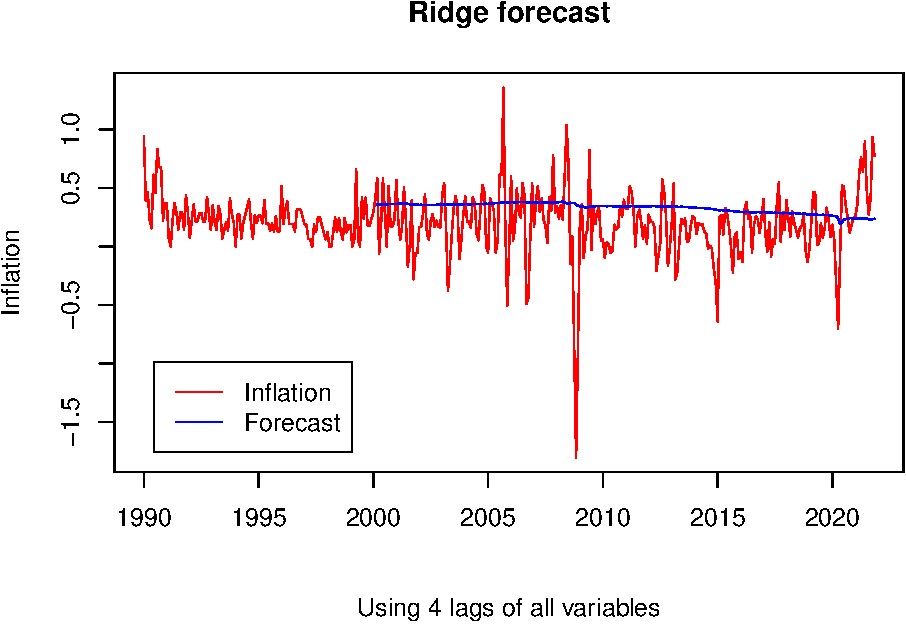
\includegraphics{Trabalho_Econo4_Q2_junto_files/figure-latex/unnamed-chunk-20-1.pdf}

\begin{Shaded}
\begin{Highlighting}[]
\CommentTok{\# Save forecasts}
\NormalTok{forecasts }\OtherTok{=} \FunctionTok{cbind.zoo}\NormalTok{(forecasts, }\AttributeTok{Ridge =}\NormalTok{ forecast1) }\SpecialCharTok{\%\textgreater{}\%}
    \FunctionTok{as.ts}\NormalTok{()}
\end{Highlighting}
\end{Shaded}

\hypertarget{lasso-regression}{%
\subsubsection{LASSO Regression}\label{lasso-regression}}

\begin{Shaded}
\begin{Highlighting}[]
\CommentTok{\# Rolling window forecasting}
\NormalTok{rolling\_window }\OtherTok{\textless{}{-}} \DecValTok{492}

\CommentTok{\# glmnet parameter}
\NormalTok{my\_alpha }\OtherTok{=} \DecValTok{1}  \CommentTok{\# LASSO}

\NormalTok{forecast1 }\OtherTok{=} \FunctionTok{list}\NormalTok{()}

\ControlFlowTok{for}\NormalTok{ (a }\ControlFlowTok{in} \DecValTok{1}\SpecialCharTok{:}\NormalTok{(}\FunctionTok{length}\NormalTok{(inflation) }\SpecialCharTok{{-}}\NormalTok{ rolling\_window)) \{}
    \CommentTok{\# get the window for training the model}
\NormalTok{    train }\OtherTok{=}\NormalTok{ data[a}\SpecialCharTok{:}\NormalTok{(a }\SpecialCharTok{+}\NormalTok{ rolling\_window }\SpecialCharTok{{-}} \DecValTok{1}\NormalTok{), ]}
    \CommentTok{\# embed}
\NormalTok{    reg\_data }\OtherTok{=} \FunctionTok{my\_embed}\NormalTok{(train)}
    \CommentTok{\# bind the embeded columns with the one{-}step{-}ahead}
    \CommentTok{\# inflation}
\NormalTok{    reg\_data }\OtherTok{=} \FunctionTok{bind\_cols}\NormalTok{(}\AttributeTok{inflation.ahead =} \FunctionTok{lead}\NormalTok{(inflation[a}\SpecialCharTok{:}\NormalTok{(a }\SpecialCharTok{+}
\NormalTok{        rolling\_window }\SpecialCharTok{{-}} \DecValTok{1}\NormalTok{)]), reg\_data)}

    \CommentTok{\# Ridge estimation}
\NormalTok{    ic\_ridge }\OtherTok{\textless{}{-}} \FunctionTok{ic.glmnet}\NormalTok{(}\AttributeTok{x =}\NormalTok{ reg\_data }\SpecialCharTok{\%\textgreater{}\%}
        \FunctionTok{na.omit}\NormalTok{() }\SpecialCharTok{\%\textgreater{}\%}
        \FunctionTok{select}\NormalTok{(}\SpecialCharTok{{-}}\NormalTok{inflation.ahead), }\AttributeTok{y =}\NormalTok{ reg\_data }\SpecialCharTok{\%\textgreater{}\%}
        \FunctionTok{na.omit}\NormalTok{() }\SpecialCharTok{\%\textgreater{}\%}
        \FunctionTok{select}\NormalTok{(inflation.ahead) }\SpecialCharTok{\%\textgreater{}\%}
        \FunctionTok{data.matrix}\NormalTok{(), }\AttributeTok{crit =} \StringTok{"bic"}\NormalTok{, }\AttributeTok{alpha =}\NormalTok{ my\_alpha)}
\NormalTok{    ridge }\OtherTok{\textless{}{-}} \FunctionTok{glmnet}\NormalTok{(}\AttributeTok{x =}\NormalTok{ reg\_data }\SpecialCharTok{\%\textgreater{}\%}
        \FunctionTok{na.omit}\NormalTok{() }\SpecialCharTok{\%\textgreater{}\%}
        \FunctionTok{select}\NormalTok{(}\SpecialCharTok{{-}}\NormalTok{inflation.ahead), }\AttributeTok{y =}\NormalTok{ reg\_data }\SpecialCharTok{\%\textgreater{}\%}
        \FunctionTok{na.omit}\NormalTok{() }\SpecialCharTok{\%\textgreater{}\%}
        \FunctionTok{select}\NormalTok{(inflation.ahead) }\SpecialCharTok{\%\textgreater{}\%}
        \FunctionTok{data.matrix}\NormalTok{(), }\AttributeTok{alpha =}\NormalTok{ my\_alpha, }\AttributeTok{lambda =}\NormalTok{ ic\_ridge}\SpecialCharTok{$}\NormalTok{lambda)}

    \CommentTok{\# Prediction}
\NormalTok{    new }\OtherTok{=}\NormalTok{ reg\_data }\SpecialCharTok{\%\textgreater{}\%}
        \FunctionTok{select}\NormalTok{(}\SpecialCharTok{{-}}\NormalTok{inflation.ahead) }\SpecialCharTok{\%\textgreater{}\%}
        \FunctionTok{tail}\NormalTok{(}\DecValTok{1}\NormalTok{)}
\NormalTok{    forecast1[a] }\OtherTok{=} \FunctionTok{predict}\NormalTok{(ridge, }\AttributeTok{newx =} \FunctionTok{data.matrix}\NormalTok{(new), }\AttributeTok{s =}\NormalTok{ ic\_ridge}\SpecialCharTok{$}\NormalTok{lambda)}
\NormalTok{\}}

\NormalTok{forecast1 }\OtherTok{=}\NormalTok{ forecast1 }\SpecialCharTok{\%\textgreater{}\%}
    \FunctionTok{unlist}\NormalTok{() }\SpecialCharTok{\%\textgreater{}\%}
    \FunctionTok{ts}\NormalTok{(}\AttributeTok{start =} \FunctionTok{start}\NormalTok{(inflation) }\SpecialCharTok{+} \FunctionTok{c}\NormalTok{(}\DecValTok{0}\NormalTok{, rolling\_window), }\AttributeTok{frequency =} \FunctionTok{frequency}\NormalTok{(inflation))}
\end{Highlighting}
\end{Shaded}

\begin{Shaded}
\begin{Highlighting}[]
\CommentTok{\# Rolling window forecasting}
\NormalTok{rolling\_window }\OtherTok{\textless{}{-}} \DecValTok{492}

\CommentTok{\# glmnet parameter}
\NormalTok{my\_alpha }\OtherTok{=} \DecValTok{1}  \CommentTok{\# LASSO}

\NormalTok{forecast1 }\OtherTok{=} \FunctionTok{list}\NormalTok{()}

\ControlFlowTok{for}\NormalTok{ (a }\ControlFlowTok{in} \DecValTok{1}\SpecialCharTok{:}\NormalTok{(}\FunctionTok{length}\NormalTok{(inflation) }\SpecialCharTok{{-}}\NormalTok{ rolling\_window)) \{}
    \CommentTok{\# get the window for training the model}
\NormalTok{    train }\OtherTok{=}\NormalTok{ data[a}\SpecialCharTok{:}\NormalTok{(a }\SpecialCharTok{+}\NormalTok{ rolling\_window }\SpecialCharTok{{-}} \DecValTok{1}\NormalTok{), ] }\SpecialCharTok{\%\textgreater{}\%}
        \FunctionTok{select}\NormalTok{(}\SpecialCharTok{{-}}\NormalTok{CPIAUCSL)}
\NormalTok{    train\_cpi }\OtherTok{=}\NormalTok{ data[a}\SpecialCharTok{:}\NormalTok{(a }\SpecialCharTok{+}\NormalTok{ rolling\_window }\SpecialCharTok{{-}} \DecValTok{1}\NormalTok{), ] }\SpecialCharTok{\%\textgreater{}\%}
        \FunctionTok{select}\NormalTok{(CPIAUCSL)}
    \CommentTok{\# embed}
\NormalTok{    reg\_data }\OtherTok{=} \FunctionTok{my\_embed}\NormalTok{(train, }\AttributeTok{n\_lags =} \DecValTok{1}\NormalTok{)}
\NormalTok{    cpi\_lags }\OtherTok{=} \FunctionTok{my\_embed}\NormalTok{(train\_cpi, }\AttributeTok{n\_lags =} \DecValTok{24}\NormalTok{)}
    \CommentTok{\# bind the embeded columns with the one{-}step{-}ahead}
    \CommentTok{\# inflation}
\NormalTok{    reg\_data }\OtherTok{=} \FunctionTok{bind\_cols}\NormalTok{(}\AttributeTok{inflation.ahead =} \FunctionTok{lead}\NormalTok{(inflation[a}\SpecialCharTok{:}\NormalTok{(a }\SpecialCharTok{+}
\NormalTok{        rolling\_window }\SpecialCharTok{{-}} \DecValTok{1}\NormalTok{)]), cpi\_lags, reg\_data) }\SpecialCharTok{\%\textgreater{}\%}
        \FunctionTok{na.omit}\NormalTok{()}

    \CommentTok{\# LASSO estimation}
\NormalTok{    ic\_lasso }\OtherTok{\textless{}{-}} \FunctionTok{ic.glmnet}\NormalTok{(}\AttributeTok{x =}\NormalTok{ reg\_data }\SpecialCharTok{\%\textgreater{}\%}
        \FunctionTok{select}\NormalTok{(}\SpecialCharTok{{-}}\NormalTok{inflation.ahead), }\AttributeTok{y =}\NormalTok{ reg\_data}\SpecialCharTok{$}\NormalTok{inflation.ahead,}
        \AttributeTok{crit =} \StringTok{"bic"}\NormalTok{, }\AttributeTok{alpha =}\NormalTok{ my\_alpha)}
\NormalTok{    lasso }\OtherTok{\textless{}{-}} \FunctionTok{glmnet}\NormalTok{(}\AttributeTok{x =}\NormalTok{ reg\_data }\SpecialCharTok{\%\textgreater{}\%}
        \FunctionTok{select}\NormalTok{(}\SpecialCharTok{{-}}\NormalTok{inflation.ahead), }\AttributeTok{y =}\NormalTok{ reg\_data}\SpecialCharTok{$}\NormalTok{inflation.ahead,}
        \AttributeTok{alpha =}\NormalTok{ my\_alpha, }\AttributeTok{lambda =}\NormalTok{ ic\_lasso}\SpecialCharTok{$}\NormalTok{lambda)}

    \CommentTok{\# Prediction}
\NormalTok{    new }\OtherTok{=}\NormalTok{ reg\_data }\SpecialCharTok{\%\textgreater{}\%}
        \FunctionTok{select}\NormalTok{(}\SpecialCharTok{{-}}\NormalTok{inflation.ahead) }\SpecialCharTok{\%\textgreater{}\%}
        \FunctionTok{tail}\NormalTok{(}\DecValTok{1}\NormalTok{)}
\NormalTok{    forecast1[a] }\OtherTok{=} \FunctionTok{predict}\NormalTok{(lasso, }\AttributeTok{newx =} \FunctionTok{data.matrix}\NormalTok{(new), }\AttributeTok{s =}\NormalTok{ ic\_lasso}\SpecialCharTok{$}\NormalTok{lambda)}
\NormalTok{\}}

\NormalTok{forecast1 }\OtherTok{=}\NormalTok{ forecast1 }\SpecialCharTok{\%\textgreater{}\%}
    \FunctionTok{unlist}\NormalTok{() }\SpecialCharTok{\%\textgreater{}\%}
    \FunctionTok{ts}\NormalTok{(}\AttributeTok{start =} \FunctionTok{start}\NormalTok{(inflation) }\SpecialCharTok{+} \FunctionTok{c}\NormalTok{(}\DecValTok{0}\NormalTok{, rolling\_window), }\AttributeTok{frequency =} \FunctionTok{frequency}\NormalTok{(inflation))}
\end{Highlighting}
\end{Shaded}

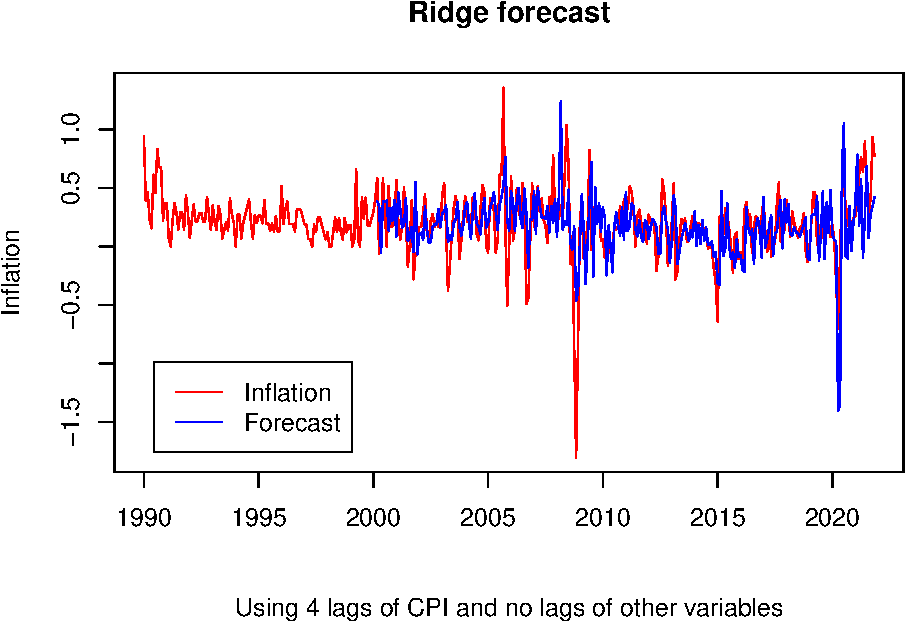
\includegraphics{Trabalho_Econo4_Q2_junto_files/figure-latex/unnamed-chunk-22-1.pdf}

\begin{Shaded}
\begin{Highlighting}[]
\CommentTok{\# Save forecasts}
\NormalTok{forecasts }\OtherTok{=} \FunctionTok{cbind.zoo}\NormalTok{(forecasts, }\AttributeTok{LASSO =}\NormalTok{ forecast1) }\SpecialCharTok{\%\textgreater{}\%}
    \FunctionTok{as.ts}\NormalTok{()}
\end{Highlighting}
\end{Shaded}

\hypertarget{item-a}{%
\subsection{Item A}\label{item-a}}

\begin{Shaded}
\begin{Highlighting}[]
\CommentTok{\# Forecasting error}
\NormalTok{error }\OtherTok{=}\NormalTok{ inflation }\SpecialCharTok{{-}}\NormalTok{ forecasts}
\NormalTok{cum\_error }\OtherTok{=} \FunctionTok{sapply}\NormalTok{(error, }\ControlFlowTok{function}\NormalTok{(x) \{}
\NormalTok{    x}\SpecialCharTok{\^{}}\DecValTok{2} \SpecialCharTok{\%\textgreater{}\%}
        \FunctionTok{cumsum}\NormalTok{()}
\NormalTok{\}) }\SpecialCharTok{\%\textgreater{}\%}
    \FunctionTok{bind\_cols}\NormalTok{(}\AttributeTok{date =} \FunctionTok{as.Date.yearmon}\NormalTok{(}\FunctionTok{time}\NormalTok{(error))) }\SpecialCharTok{\%\textgreater{}\%}
    \FunctionTok{setNames}\NormalTok{(}\FunctionTok{c}\NormalTok{(}\StringTok{"AR"}\NormalTok{, }\StringTok{"AR\_PC"}\NormalTok{, }\StringTok{"Ridge"}\NormalTok{, }\StringTok{"LASSO"}\NormalTok{, }\StringTok{"date"}\NormalTok{))}
\end{Highlighting}
\end{Shaded}

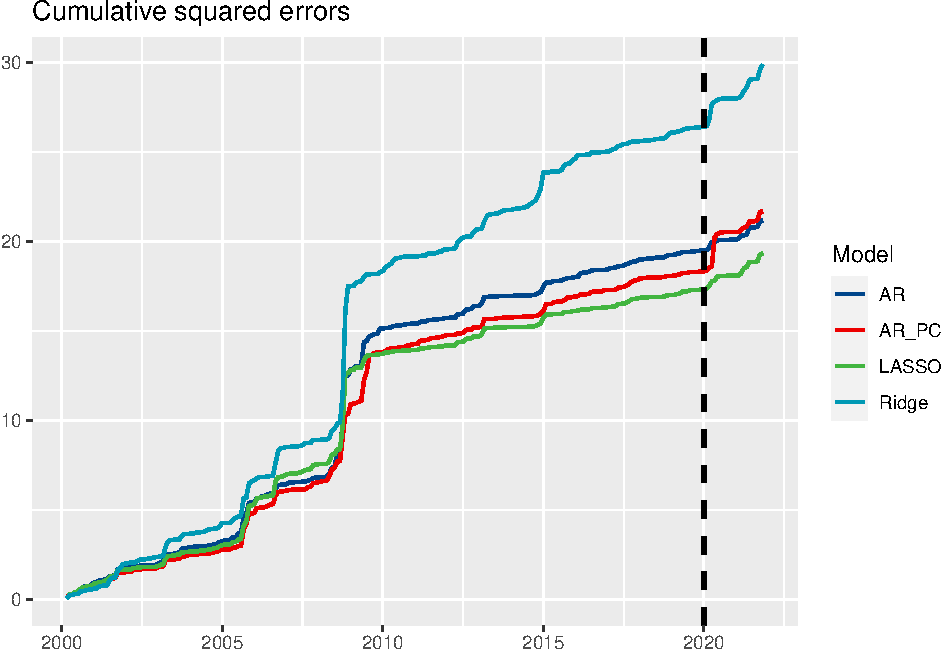
\includegraphics{Trabalho_Econo4_Q2_junto_files/figure-latex/unnamed-chunk-25-1.pdf}

\begin{Shaded}
\begin{Highlighting}[]
\CommentTok{\# Save data for Question 3}
\FunctionTok{save}\NormalTok{(data, inflation, forecasts, }\AttributeTok{file =} \StringTok{"data/Q2\_objects.Rda"}\NormalTok{)}
\FunctionTok{write.csv}\NormalTok{(forecasts, }\AttributeTok{file =} \StringTok{"forecasts.csv"}\NormalTok{)}
\FunctionTok{write.csv}\NormalTok{(cum\_error, }\AttributeTok{file =} \StringTok{"cum\_error.csv"}\NormalTok{)}
\end{Highlighting}
\end{Shaded}


\end{document}
